\section{stabilizer.c File Reference}
\label{stabilizer_8c}\index{stabilizer.c@{stabilizer.c}}
{\tt \#include $<$stdio.h$>$}\par
{\tt \#include $<$stdlib.h$>$}\par
{\tt \#include \char`\"{}globals.h\char`\"{}}\par
{\tt \#include \char`\"{}stabilizer.h\char`\"{}}\par
{\tt \#include \char`\"{}adc.h\char`\"{}}\par
{\tt \#include \char`\"{}motor\_\-pwm.h\char`\"{}}\par


Include dependency graph for stabilizer.c:\begin{figure}[H]
\begin{center}
\leavevmode
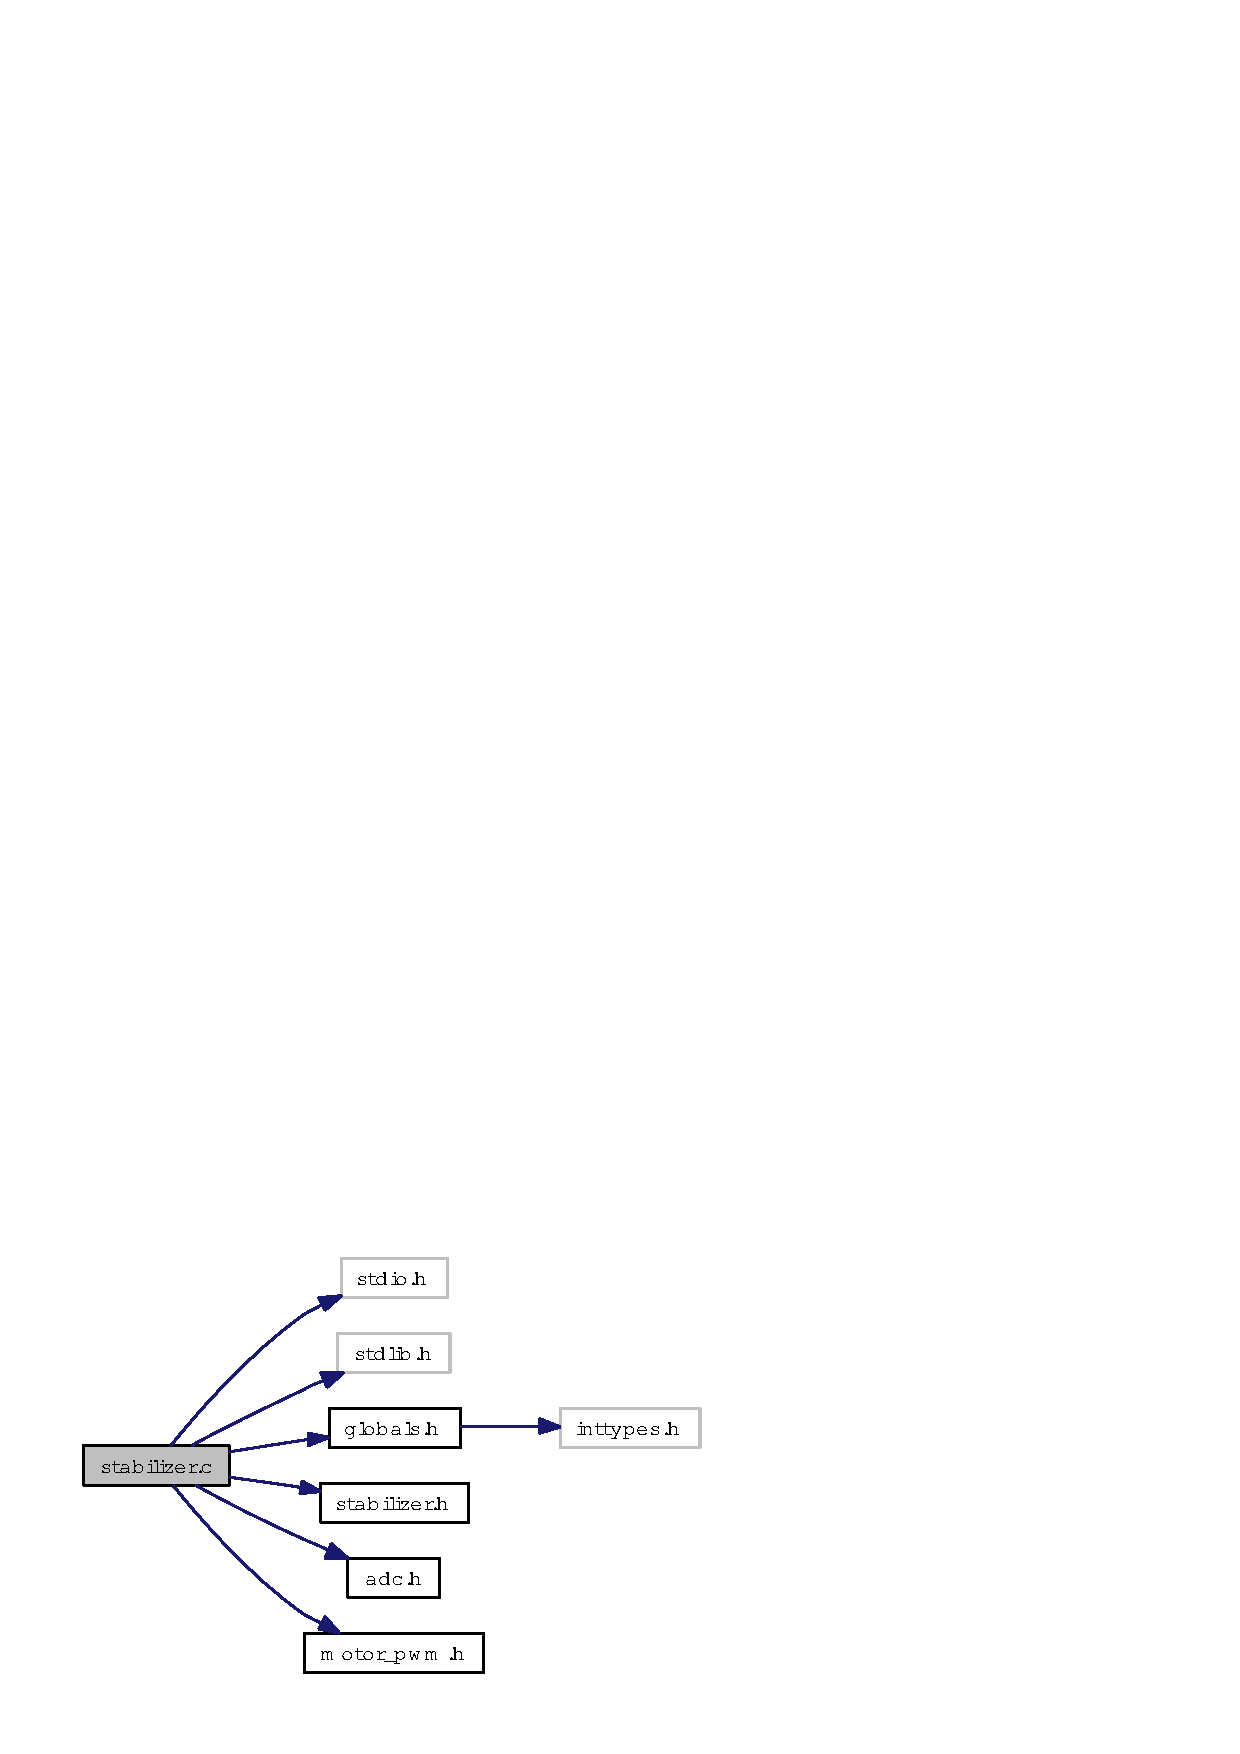
\includegraphics[width=170pt]{stabilizer_8c__incl}
\end{center}
\end{figure}
\subsection*{Functions}
\begin{CompactItemize}
\item 
void {\bf stabilizer\_\-loop} (void)
\end{CompactItemize}


\subsection{Function Documentation}
\index{stabilizer.c@{stabilizer.c}!stabilizer_loop@{stabilizer\_\-loop}}
\index{stabilizer_loop@{stabilizer\_\-loop}!stabilizer.c@{stabilizer.c}}
\subsubsection{\setlength{\rightskip}{0pt plus 5cm}void stabilizer\_\-loop (void)}\label{stabilizer_8c_cc3a7bb7e4532b65fe366e14f3778f86}




Definition at line 45 of file stabilizer.c.

References accl\_\-high\_\-samples, accl\_\-low\_\-samples, ACCL\_\-SAMPLES\_\-BUFSIZE, ACCL\_\-TO\_\-DEGREE\_\-FACTOR, adc\_\-sel\_\-channel(), ADC\_\-STEERING\_\-1, CUR\_\-SPEED\_\-FACTOR, gyro1\_\-samples, GYRO1\_\-SAMPLES\_\-BUFSIZE, GYRO1\_\-ZERO\_\-VALUE, GYRO\_\-TO\_\-OMEGA\_\-FACTOR, K\_\-ANGLE, K\_\-OMEGA, PI, PWM\_\-RESOLUTION, read\_\-adc(), set\_\-motor1(), set\_\-motor2(), SET\_\-POINT, STEERING\_\-RESPONSIVENESS, STEERING\_\-ZERO\_\-POINT, and uart\_\-puts().

Here is the call graph for this function:\begin{figure}[H]
\begin{center}
\leavevmode
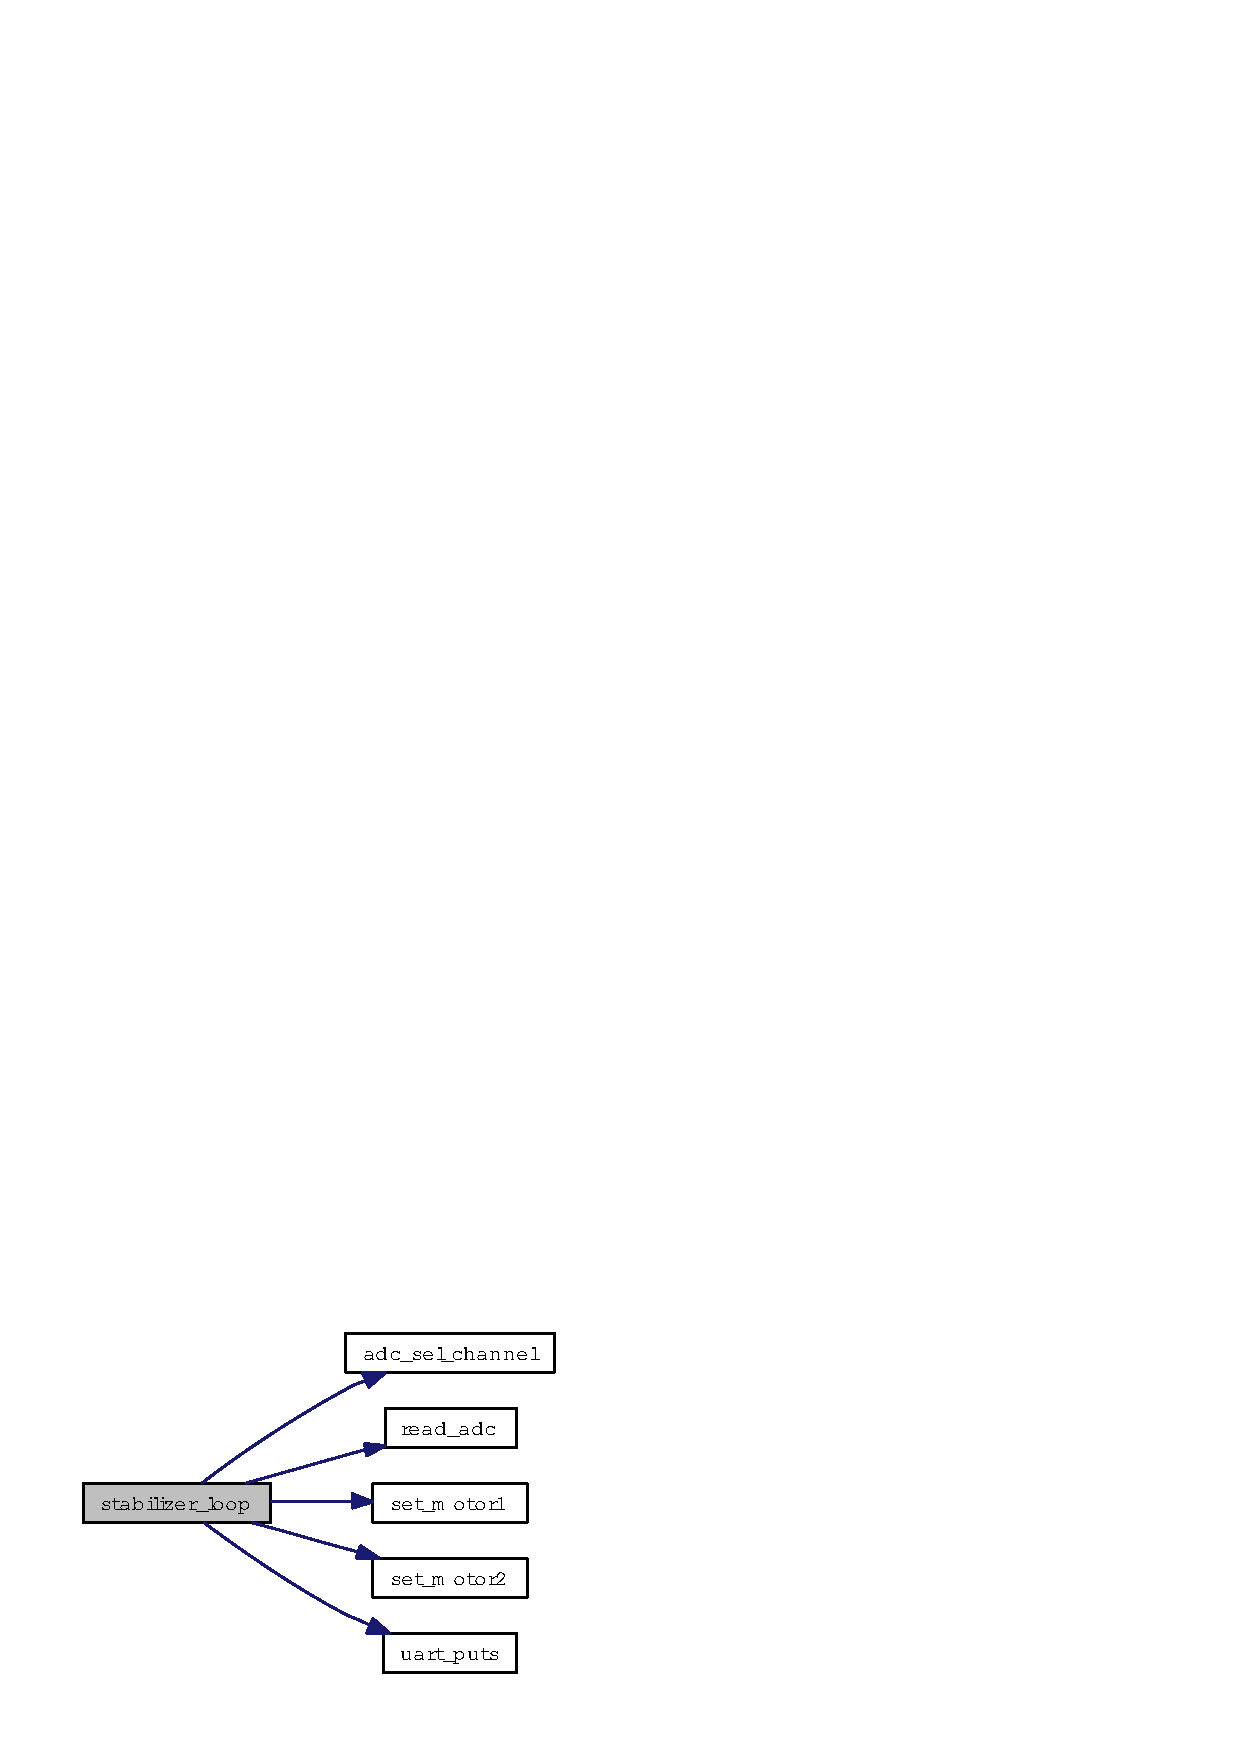
\includegraphics[width=135pt]{stabilizer_8c_cc3a7bb7e4532b65fe366e14f3778f86_cgraph}
\end{center}
\end{figure}
